\chapter{绪论}\label{chap:kondo}

\section{冷原子概述}


杂质物理,其中少体体系与多体体系

\section{冷原子基本实验技术}

冷却囚禁费米子技术

光晶格

Feshbach resonance

Confiment induced resonance

\section{费米子少体体系}\label{sec:fewbody}
伴随着冷原子平台实验技术的进步,各个凝聚态研究领域掀起了不同程度的热潮。其中少体物理的研究领域有了较大进展。得益于实验中少量原子体系的
制备、调控与测量,少体物理中很多概念诸如少体束缚态、费米化等理论概念不断地在冷原子实验中被观测到,并进而引发了冷原子特性平台下相关少体物理的理论研究。实际的冷原子少体体系中几个原子被束缚在势阱中,因此我们的内容也主要限制在束缚势阱中的少体体系实验与理论研究进展,以期为接下来的研究提供启发,更细致全面的review可推荐\cite{sowinski2019one,blume2012few},本章还不会涉及Efimov物理,相关review参见\cite{nielsen2001three,braaten2006universality,KohlerMolFRRMP}。由于原子间全同性原理,我们将围绕玻色少体体系与费米少体体系分别展开。束缚的原子数可控程度越来越高,体系的维度可以通过各向异性的势阱实现,原子之间的相互作用均可以调节,从极弱到极强,从吸引到排斥。进一步选取不同的混合体系带来质量比的可调节性,这些丰富的可调节实验条件为少体体系带来丰富的物理。


\begin{comment}
\subsection{玻色子少体}

可控少体玻色子实验

少体物理之所以重要很大原因在于存在严格解。对于量子力学发展初期的谐振子严格解与氢原子模型严格解的理解,几乎构成了我们理解量子力学的基石。进一步地,
在玻色子少体体系中,无相互作用极限下体系处于BEC极限。所有的玻色子位于体系的基态。而一旦打开玻色子之间相互作用之后,新奇的物理现象就出现了。早在1960年,M. Girardeau提出对于玻色子体系:
\begin{equation}
\hat{\mathcal{H}}=\sum_{i=1}^{N}\left[-\frac{1}{2} \frac{\partial^{2}}{\partial x_{i}^{2}}+\frac{1}{2} x_{i}^{2}\right]+g \sum_{i<j} \delta\left(x_{i}-x_{j}\right)
\end{equation}
在强排斥极限$g\to+\infty$下等价于新的带有边界条件的无相互作用哈密顿量:
\begin{equation}
\begin{split}
\hat{\mathcal{H}}&=\sum_{i=1}^{N}\left[-\frac{1}{2} \frac{\partial^{2}}{\partial x_{i}^{2}}+\frac{1}{2} x_{i}^{2}\right]\\
&\quad \phi_{x_i=x_j}=0\\
\end{split}
\end{equation}
进一步E. Lieb与找到了整个相互作用区间的严格解。Petrov研究了细香烟类型的BEC低温强相互作用下类似于T-G气体。不过上述理论都是基于自由空间,冷原子实验中通常伴随着外界的势阱。2001年Girardeau M D与合作者研究了谐振子外势存在下,强排斥N玻色子体系基态波函数可以写为Jastrow形式:
\begin{equation}
\phi(\boldsymbol{r})=C_{N}\left(\prod^{N} \prod^{N}\left|x_{i}-x_{j}\right|\right) \mathrm{e}^{-\sum_{i} x_{i}^{2} / 2}
\end{equation}
进一步,这个体系的单粒子密度矩阵:
\begin{equation}
\rho^{(1)}\left(x, x^{\prime}\right)=\int \phi\left(x, \ldots, x_{N}\right) \phi\left(x^{\prime}, \ldots, x_{N}\right) \mathrm{d} x_{2} \ldots \mathrm{d} x_{N}
\end{equation}
其对角部分为体系的密度分布,换到动量空间为:
\begin{equation}
n(k)=\frac{1}{2 \pi} \int \mathrm{d} x \int \mathrm{d} x^{\prime} \rho\left(x, x^{\prime}\right) \exp \left[-\mathrm{i} k\left(x-x^{\prime}\right)\right]
\end{equation}
对于有5个粒子的少体体系,其密度分布如图所示:
\begin{figure}[!htbp]
    \centering
    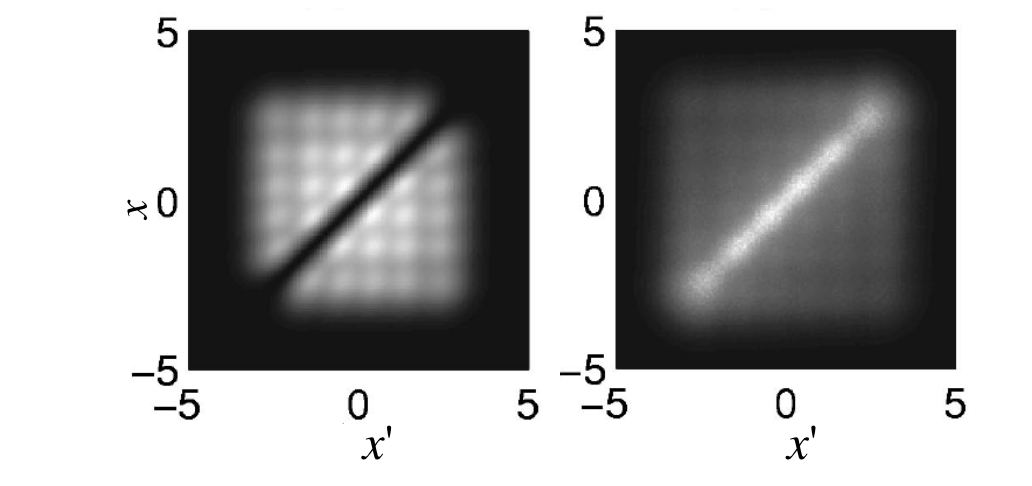
\includegraphics[width=0.6\textwidth]{chap1tgrho.png}
    \bicaption{摘自1D tg rho}{Reprinted from 1D tg rho}
    \label{chap1tgrho}
\end{figure}
不仅限于强相互作用极限,在趋向于这个极限的过程,利用严格解的办法{\color{red}Deuretzbacher F给出了少体体系费米化的过程}。
\begin{figure}[!htbp]
    \centering
    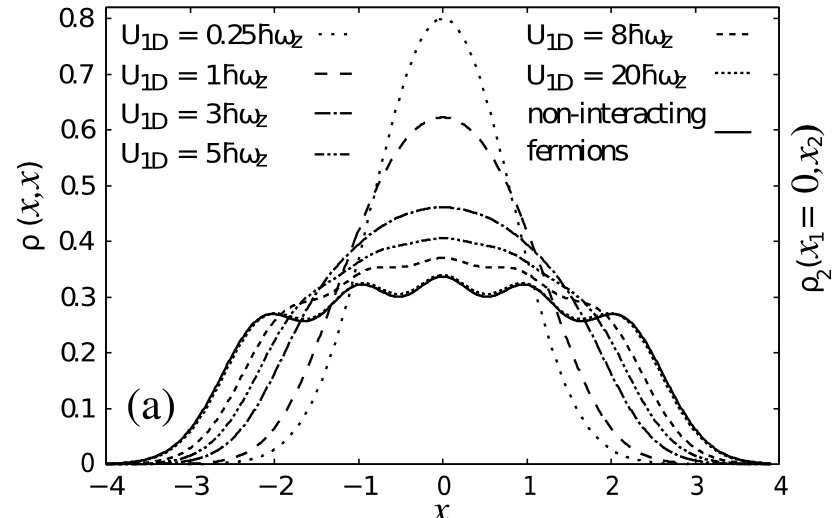
\includegraphics[width=0.6\textwidth]{chap1tgn.png}
    \bicaption{摘自1D tg n}{Reprinted from 1D tg n}
    \label{chap1tgn}
\end{figure}
最终T-G气体在实验中被观测到。
\end{comment}

\subsection{费米少体实验}
实验中最早制备出费米子少体体系可以追溯到2005年,在较深的光晶格体系中观测到两费米子形成的分子态\cite{greiner2002quantum,EsslingerFermiSea,Esslinger1DMol,Esslinger3DMol,Ospelkaus3DMol,Hecker3DMol,SalaCIRMol}。如图~\ref{chap1mol}~所示,
\begin{figure}[!htbp]
    \centering
    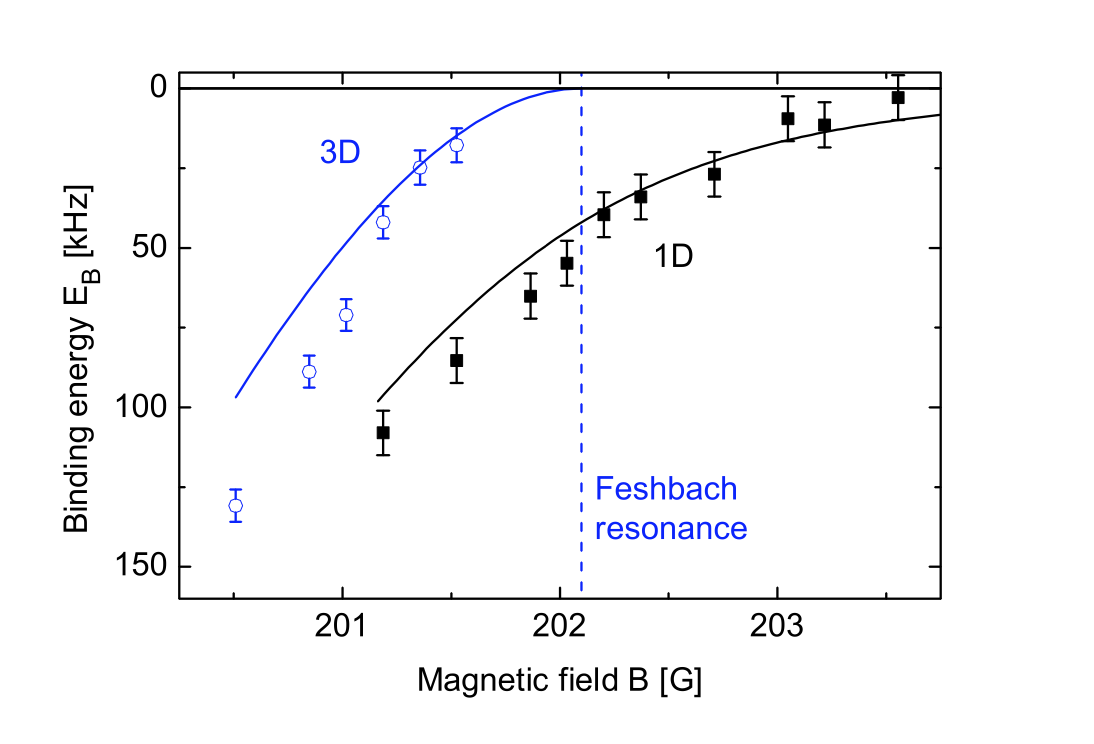
\includegraphics[width=0.6\textwidth]{chap1mol.png}
    \bicaption{摘自 Esslinger1DMol}{Reprinted Esslinger1DMol}
    \label{chap1mol}
\end{figure}

然后沿着另外一个思路,精确制备少体体系\cite{SerwaneDeterministic,WenzFermiSeaOnebyOne,zurn2012fermionization,Zurn2013Pairing,MurmannSpinChain,MurmannTwoFermionDoubleWell,RontaniTunneling}。

少体实验自旋\cite{pagano2014one}


\subsection{费米少体理论}

少体物理之所以重要是因为可以提供一个可理解的物理图像,甚至某些特殊体系存在严格解。这些少体图像成了我们理解实验的基石。在冷原子领域,有两个经典的两体图像,分别是:自由空间s波散射图像与谐振子势场下s波相互作用两体严格解。由于本节内容关在存在外势的相关少体物理,因此我们从介绍后者出发。

1998年T. Busch给出了又一个少体体系严格解:任意维度下两个全同玻色子在谐振子势场下的能谱。虽然是玻色子体系,但是这个严格解对费米子体系同样重要,我们以一维为例简单介绍,系统的哈密顿量可以写为:
\begin{equation}
\hat{\mathcal{H}}=-\frac{\hbar}{2 m}\left(\frac{\partial^{2}}{\partial x^{2}}+\frac{\partial^{2}}{\partial y^{2}}\right)+\frac{m \omega^{2}}{2}\left(x^{2}+y^{2}\right)+g \delta(x-y)
\end{equation}
其中$m$为全同玻色子的质量,$\omega$为谐振子势场的特征频率。引入一维散射长度$g= -\frac{2\hbar^2}{m}\cdot\frac{1}{a}$并分离质心运动与相对运动$R = \frac{x+y}{\sqrt{2}}, \quad X = \frac{x-y}{\sqrt{2}}$
得到$\hat{\mathcal{H} } = \hat{\mathcal{H}}_R+ \hat{\mathcal{H}}_X$:
\begin{equation}
\begin{aligned}
&\mathcal{H}_{R}=-\frac{1}{2} \frac{\mathrm{d}^{2}}{\mathrm{~d} R^{2}}+\frac{1}{2} R^{2} \\
&\mathcal{H}_{X}=-\frac{1}{2} \frac{\mathrm{d}^{2}}{\mathrm{~d} X^{2}}+\frac{1}{2} X^{2}+\frac{g}{\sqrt{2}} \delta(X)
\end{aligned}
\end{equation}
$mathcal{H}_{X}$在谐振子基矢下对角化,其中奇宇称的谐振子能级不受影响仍为$(2n+\frac{1}{2})\hbar\omega$。偶宇称的本征解能量$E_n$满足自洽方程为:
\begin{equation}
	-g \Gamma\left(\frac{1-2 E_{k}}{4}\right)=2 \sqrt{2} \Gamma\left(\frac{3-2 E_{k}}{4}\right)
\end{equation}
相应的本征波函数为:
\begin{equation}
	\Psi_{k}(X)=N_{k} \mathrm{e}^{-X^{2} / 2} \mathrm{U}\left(\frac{1-2 E_{k}}{4}, \frac{1}{2}, X^{2}\right)
\end{equation}
当相互作用$g\to\infty$时候:
\begin{equation}
\begin{split}
	E_k &\to (2k+1+1/2)\hbar\omega\\
	\Psi_{k}(X) &\to \psi_{2k+1}(X)\cdot sign(X)\\
\end{split}
\end{equation}
其中$\psi_{2k+1}(X)$为谐振子第$2k+1$个本征波函数。整个系统的能谱如图~\ref{chap1fig1}~所示
\begin{figure}[!htbp]
    \centering
    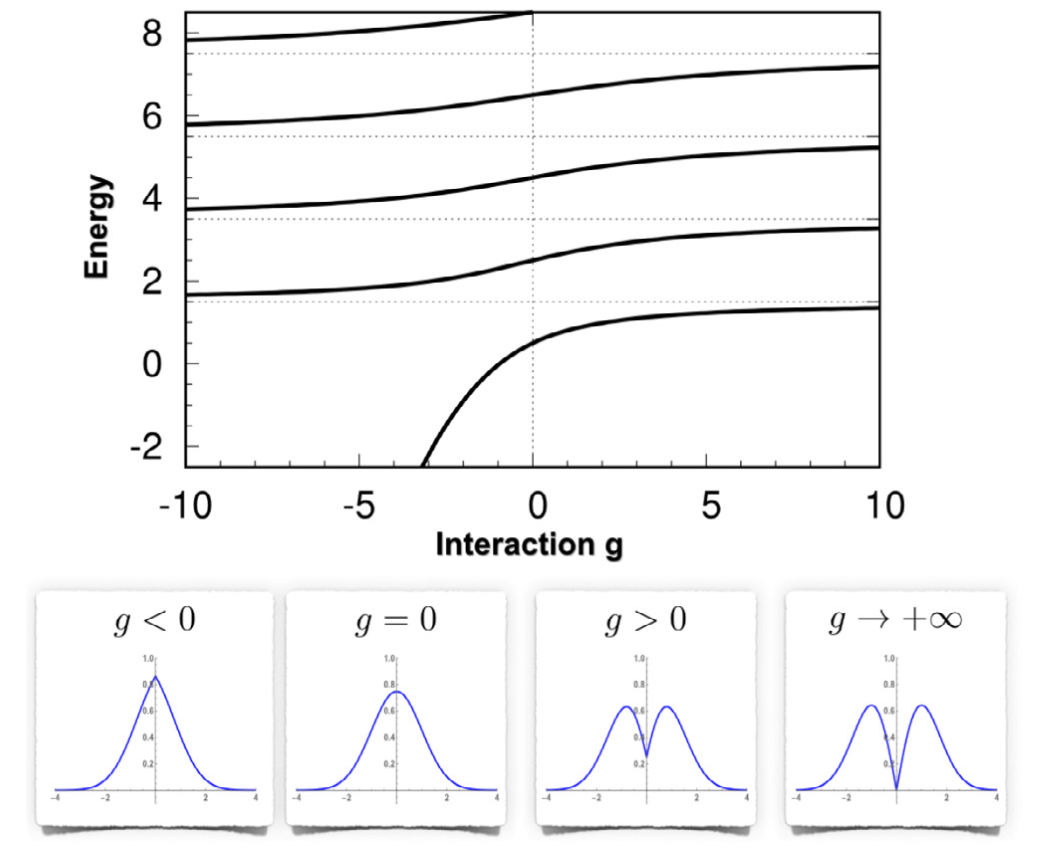
\includegraphics[width=0.6\textwidth]{chap1fig1.png}
    \bicaption{摘自1D少体势阱}{Reprinted from 1Dfewtrap}
    \label{chap1fig1}
\end{figure}
其中当$g\to-\infty$时候,基态能量渐近行为是$E_g\to-\frac{g^2}{2}$,称为lower branch。其余的随着$g\to\infty$本征能量饱和在奇数谐振子能量的态称为upper branch。这个少体体系的严格解在后续的实验与理论发展中起了很重要的做用。

{\color{red}后续有一些进一步的推广。}

2体:1D, 2D, 3D Busch l=0,l>0 及一些准一维扩展。动力学 \cite{Idziaszek2bdynamics}



如果在两体体系中再加入一个费米子,我们记为$\uparrow\downarrow\uparrow$的费米子三体体系,仅在不同自旋费米子之间有s波散射相互作用\cite{OlshaniiRigorous2001,Petrov2003unitary3b,Fleix2006prlunitary3b,Felix2006praunitary3b,LmDuan2007levelcrossing,Stetcu2007,Blume2008,Blume2010,Xiaji2009prl,Xiaji20103b,Rittenhouse2010green}。我们用Bethe-Peierls条件代替:
\begin{equation}
\psi\left(\mathbf{r}_{1}, \mathbf{r}_{2}, \mathbf{r}_{3}\right)=\left(\frac{1}{r_{i j}}-\frac{1}{a}\right) A\left(\mathbf{R}_{i j}, \mathbf{r}_{k}\right)+O\left(r_{i j}\right)
\end{equation}
其中$r_{i j} \equiv\left|\mathbf{r}_{i}-\mathbf{r}_{j}\right| \rightarrow 0$,$\mathbf{R}_{ij}$为两原子的质心位置。

这种体系的求解通常借助于HyperSphere框架,先引入Jacobi坐标:
\begin{equation}
\begin{split}
\Vector{r}&=\Vector{r}_{2}-\Vector{r}_{1}\\
\boldsymbol{\rho}&=\left(2 \mathbf{r}_{3}-\mathbf{r}_{1}-\mathbf{r}_{2}\right) / \sqrt{3}\\
\Vector{C}&=\left(\Vector{r}_{1}+\Vector{r}_{2}+\Vector{r}_{3}\right) / 3\\
\end{split}
\end{equation}
然后定义Hyperradius与Hyperangle:
\begin{equation}
\begin{split}
R&=\sqrt{\left(r^{2}+\rho^{2}\right) / 2}\\
\alpha&=\arctan (r / \rho)\\
\end{split}
\end{equation}
这时候谐振子外势只出现在$R$的薛定谔方程中。考虑波函数形式:
\begin{equation}
\psi\left(\mathbf{r}_{1}, \mathbf{r}_{2}, \mathbf{r}_{3}\right)=\psi_{\mathrm{c} . \mathrm{m} .}(\mathbf{C}) F(R)(1+\hat{Q}) \frac{1}{r \rho} \varphi(\alpha) Y_{l}^{m}(\boldsymbol{\rho} / \rho)
\end{equation}
其中$Y_l^m$为角动量为l的球谐函数。l为三体内部相对角动量。将上式带入薛定谔方程得到$\alpha$满足:
\begin{equation}
\begin{gathered}
-\varphi^{\prime \prime}(\alpha)+\frac{l(l+1)}{\cos ^{2} \alpha} \varphi(\alpha)=s^{2} \varphi(\alpha) \\
\varphi(\pi / 2)=0 \\
\varphi^{\prime}(0)+\eta(-1)^{l} \frac{4}{\sqrt{3}} \varphi(\pi / 3)=0
\end{gathered}
\end{equation}
其中$\eta=-1$。对任意l,可以解得一系列$s_{l,n},n=0,1,2,3...$均为实数。如图~\ref{Sv}
\begin{figure}[!htbp]
    \centering
    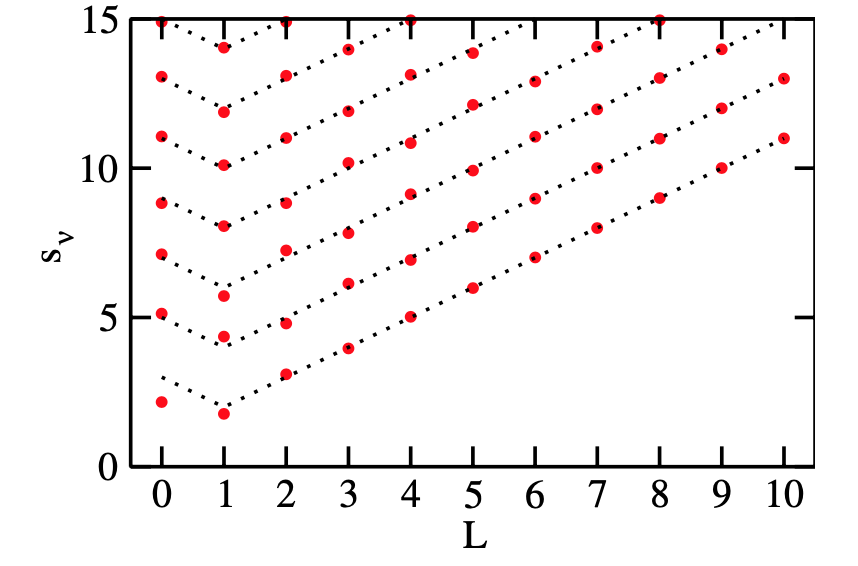
\includegraphics[width=0.7\textwidth]{chap1Sv.png}
    \bicaption{摘自Fleix2006prlunitary3bPRL}{Reprinted}
    \label{Sv}
\end{figure}
将解到的$s_{l,n}$带入:
\begin{equation}
\left[-\frac{\hbar^{2}}{2 m}\left(\frac{d^{2}}{d R^{2}}+\frac{1}{R} \frac{d}{d R}\right)+U(R)\right] F(R)=\left(E-E_{\mathrm{c} . \mathrm{m} .}\right) F(R)
\end{equation}
其中$U(R)=\hbar^{2} s^{2} /\left(2 m R^{2}\right)+m \omega^{2} R^{2} / 2$。即可求得三体本征解。基于上述框架当s波相互作用处于幺正极限$a\to+\infty$时候能谱为:
\begin{equation}
E=E_{\mathrm{c} . \mathrm{m} .}+\left(s_{l, n}+1+2 q\right) \hbar \omega
\end{equation}

Duan用格林函数的方法数值求解了整个相互作用区间。
\begin{equation}
\begin{aligned}
\Psi(\mathbf{x}, \mathbf{y})=& \int d \mathbf{x}^{\prime} d \mathbf{y}^{\prime} G_{E}^{(2)}\left(\mathbf{x}, \mathbf{y} ; \mathbf{x}^{\prime}, \mathbf{y}^{\prime}\right)\times \sum_{\pm} \frac{\mp \hbar^{2} f\left(\mathbf{r}^{\prime}{ }_{\perp, \pm}\right)}{m_{0}} \delta\left(\mathbf{r}^{\prime}{ }_{\pm}\right)\\
G_{E}^{(2)}\left(\mathbf{x}, \mathbf{y} ; \mathbf{x}^{\prime}, \mathbf{y}^{\prime}\right)&=\sum_{\lambda_{1} \lambda_{2}} \frac{\psi_{\lambda_{1}}(\mathbf{x}) \psi_{\lambda_{2}}(\mathbf{y}) \psi_{\lambda_{1}}^{*}\left(\mathbf{x}^{\prime}\right) \psi_{\lambda_{2}}^{*}\left(\mathbf{y}^{\prime}\right)}{E_{\lambda_{1}}+E_{\lambda_{2}}-E}\\
\end{aligned}
\end{equation}
其中$\psi_\lambda(\Vector{r}) = R_{nl}(r)Y_l^m(\theta,\phi)$,$\lambda = (n,l,m),n=0,1,2...,l=0,1,2...$,边界条件为:
\begin{equation}
\Psi(\mathbf{x}, \mathbf{y}) \simeq \mp \frac{f\left(\mathbf{r}_{\perp, \pm}\right)}{4 \pi \mathbf{r}_{\pm}}\left(1-\frac{\mathbf{r}_{\pm}}{a}\right) \text { for } \mathbf{r}_{\pm} \rightarrow 0
\end{equation}
其能谱如图~\ref{duan}~所示,通过跟两体能量的比较作者进一步发现了能级交叉。
\begin{figure}[!htbp]
    \centering
    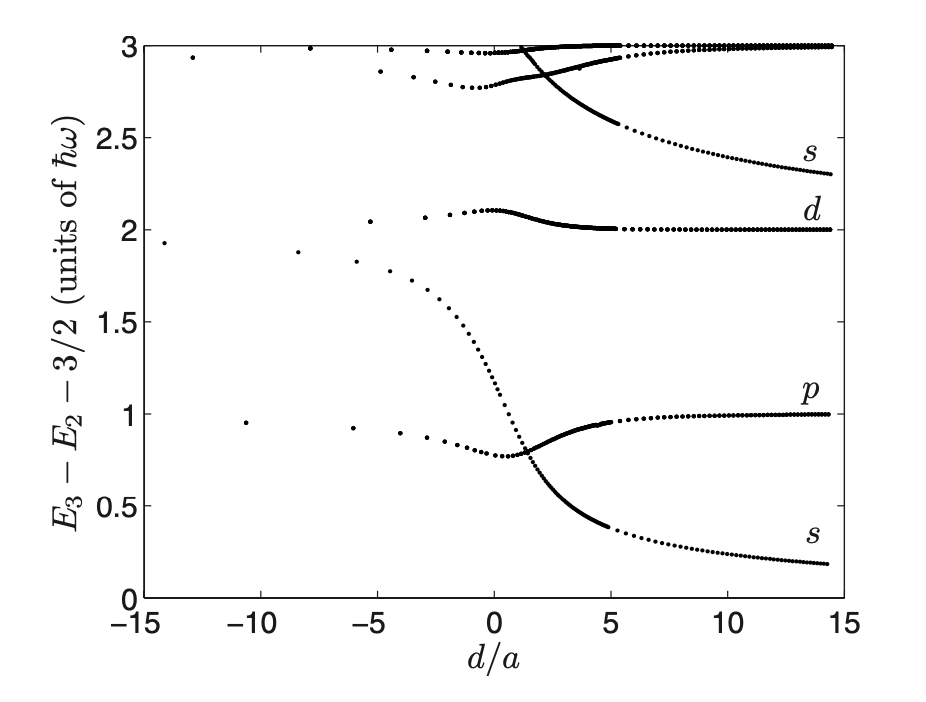
\includegraphics[width=0.7\textwidth]{chap1duan.png}
    \bicaption{摘自Fleix2006prlunitary3bPRL}{Reprinted}
    \label{duan}
\end{figure}

后续研究者Xiaji则用2b本征波函数展开求解了整个相互作用区间的严格解,采用的波函数为:
\begin{equation}
\begin{split}
\psi_{3 b}^{\mathrm{rel}}(\mathbf{r}, \rho)&=\left(1-\mathcal{P}_{13}\right) \chi(\mathbf{r}, \rho)\\
\chi(\mathbf{r}, \rho)&=\sum a_{n} \psi_{2 b}^{\mathrm{rel}}\left(r ; v_{l, n}\right) R_{n l}(\rho) Y_{l}^{m}(\hat{\rho})\\
\end{split}
\end{equation}
其中$\psi_{2 b}^{\mathrm{rel}}$代表费米子1,2相对运动的波函数,对应能量为$E_{2b}=(2v_{l,n}+3/2)\hbar\omega$,而$R_{nl}(\rho Y^m_l(\hat{\rho}))$,其中$l,m$是系统的好量子数,代表了相对角动量与其沿z方向的分量。其物理图像非常清晰,将其中一个$\uparrow$费米子与$\downarrow$费米子结合在一起成为二聚体,第三个费米子相对于这个二聚体的运动由$a_n$所描述。最终求解方程:
\begin{equation}
\begin{split}
&\frac{2 \Gamma\left(-v_{l, n}\right)}{\Gamma\left(-v_{l, n}-1 / 2\right)} a_{n}+\frac{(-1)^{l}}{\sqrt{\pi}} \sum_{n^{\prime}} C_{n n^{\prime}} a_{n^{\prime}}=\left(\frac{d}{a}\right) a_{n}\\
&C_{n n^{\prime}} \equiv \int_{0}^{\infty} \rho^{2} d \rho R_{n l}(\rho) R_{n^{\prime} l}\left(\frac{\rho}{2}\right) \psi_{2 b}^{\mathrm{rel}}\left(\frac{\sqrt{3} \rho}{2} ; v_{l, n^{\prime}}\right)\\
\end{split}
\end{equation}
其能谱如图~\ref{xiaji}~所示。
\begin{figure}[!htbp]
    \centering
    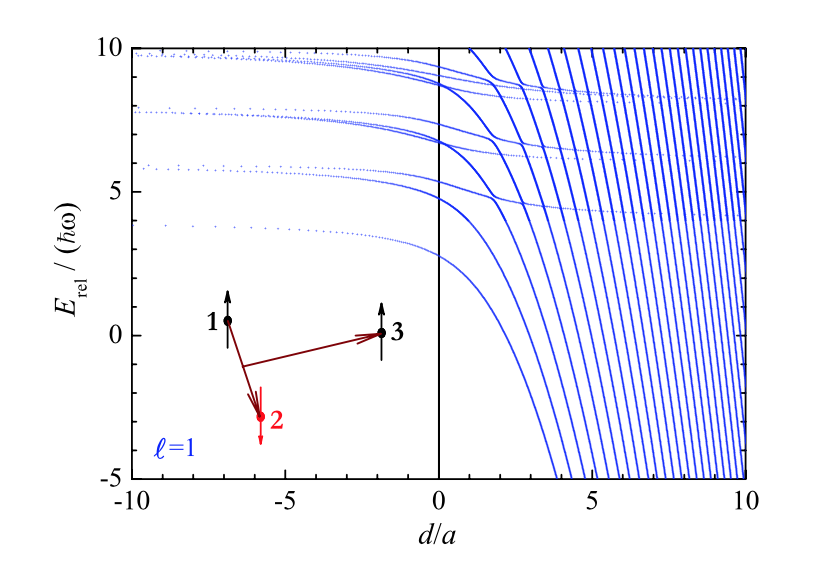
\includegraphics[width=0.7\textwidth]{chap1xiaji.png}
    \bicaption{摘自Fleix2006prlunitary3bPRL}{Reprinted}
    \label{xiaoji}
\end{figure}
与此同时,研究者Xiaji还研究了二维体系下,三体精确解,采用类似的办法,
\begin{equation}
\begin{split}
\psi_{3 f}^{r e l}&=\left(1-\mathcal{P}_{13}\right) \chi(\mathbf{r}, \vec{\rho})\\
\chi(\mathbf{r}, \vec{\rho})&=\sum_{n} a_{n}^{f} \psi_{2 p}^{r e l}\left(\mathbf{r} ; \nu_{m, n}\right) R_{n m}(\rho) \frac{e^{i m \varphi}}{\sqrt{2 \pi}}\\
\end{split}
\end{equation}
得到整个相互作用的能谱。

进一步Blume研究了从三维到二维一维的渡越,通过研究各项异性的谐振子束缚势能,作者系统地求得了体系的能谱。

而在严格一维体系里面,三费米子的严格求解则由\cite{Rittenhouse2010green,d2014three,loft2015variational,andersen2016interpolatory,bellotti2017comparing}给出。
采用的波函数为:
\begin{equation}
\begin{split}
\psi_{3 F}(x, y)&=\left(1-\boldsymbol{P}_{13}\right) \Omega(x, y)\\
\Omega(x, y)&=\sum_{n=0}^{\infty} a_{n} \psi_{n}^{2b}(x) R_{n}(y)\\
\psi_{n}^{2b}(x)&=\Gamma\left(-v_{n}\right) \mathrm{e}^{-\frac{x^{2}}{2}} U\left(-v_{n}, \frac{1}{2}, x^{2}\right)\\
\end{split}
\end{equation}
其中$\psi_{n}^{2b}(x)$为两体相互作用在谐振势中的解,$R_{n}(y)$为谐振子的本征解。类似地,带入到Bethe–Peierls边界条件中得到耦合方程:
\begin{equation}
\begin{aligned}
&2 g \sum_{n} a_{n}\left[\sqrt{\pi} \frac{\Gamma\left(-v_{n}\right)}{\Gamma\left(-v_{n}+1 / 2\right)} R_{n}(y)-\psi_{n}\left(\frac{\sqrt{3}}{2} y\right) R_{n}\left(-\frac{y}{2}\right)\right] \\
&=-4 \sqrt{\pi} \sum_{n} a_{n} R_{n}(y)
\end{aligned}
\end{equation}
相应地能谱如图~\ref{1d3b}~所示。
\begin{figure}[!htbp]
    \centering
    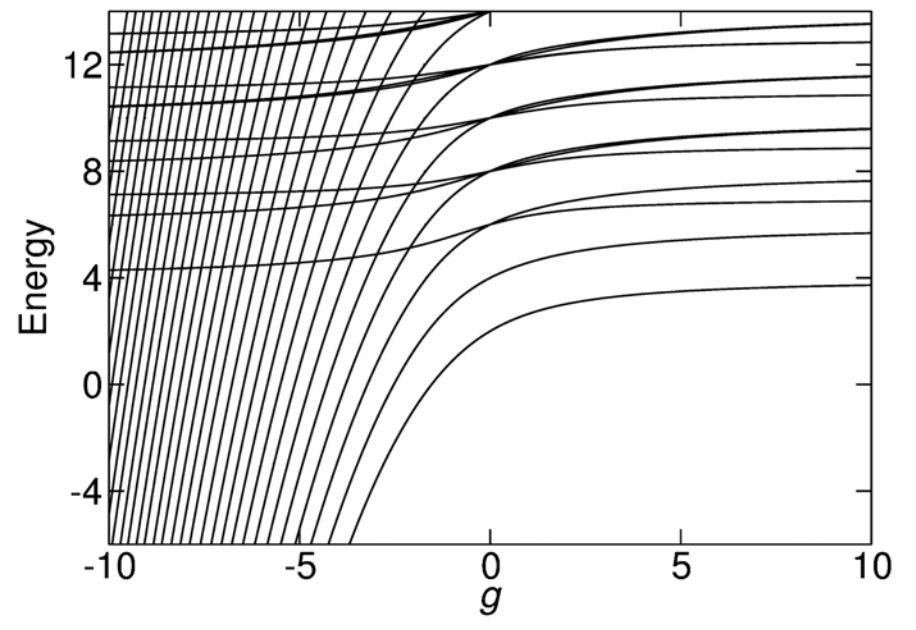
\includegraphics[width=0.7\textwidth]{chap11d3b.png}
    \bicaption{摘自Fleix2006prlunitary3bPRL}{Reprinted}
    \label{1d3b}
\end{figure}


在严格一维体系中,很多问题通过bethe ansatz可以得到严格解,但是bethe ansatz的结果很多时候物理上并不直观。仅在某些极限下有清楚的物理图像,在这其中,得益于实验上的启发,自旋链模型研究颇多。从两体能谱我们得知费米子在$g\to\infty$时有upper branch,
\begin{figure}[!htbp]
    \centering
    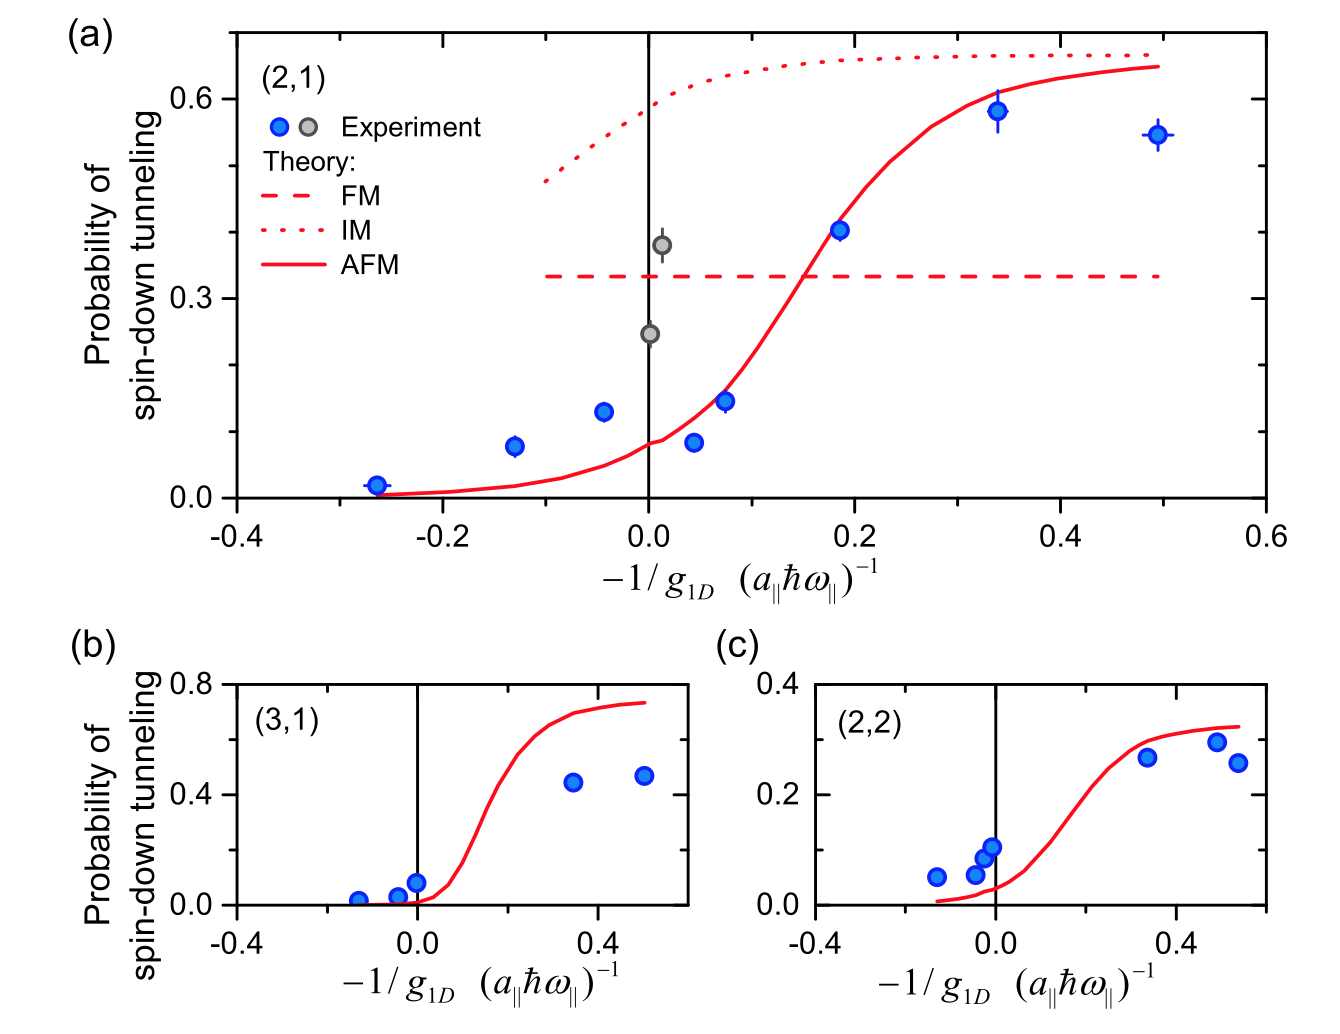
\includegraphics[width=0.7\textwidth]{chap1spinchain.png}
    \bicaption{摘自Fleix2006prlunitary3bPRL}{Reprinted}
    \label{spinchain}
\end{figure}


在三体中继续增加一个费米子到四体体系则有两种加法,一种是3+1,一种是2+2,三维、二维、一维有研究。




1D少体高自旋少体,自旋链

1D两体2010M. D. Girardeau. 

1D SOC 2体,

1D 少体极化子,围绕Wenz的science实验,一系列理论

陈老师1D严格解 TG limit。一维自旋链崔老师

Intermediate interactions1D,ED in Fock Basis。选取适当的高能态得到好的收敛性。

Zinner变分ansatz 1D

FermionParing 少体in1D



有了上面介绍的量子少体研究进展,将有几个可扩展的方向,比如改变相互作用,dipole、库伦、以及自旋交换相互作用,而自旋交换相互作用这将是下一章节介绍的。

\section{自旋交换相互作用}\label{sec:spin-exchange}

\subsection{自旋交换实验}
在超冷原子实验平台中,原子整体作为基本粒子,但是具有内禀自由度。分为内部电子轨道自由度和核自旋自由度。在冷原子实验平台发展初期,冷却囚禁的原子主要集中在碱金属一族,最外层只有一个电子。后续随着实验技术的进步,碱土金属一族的原子进入到大家的视野{\color{red} AE原子体系制备 }。这类冷原子最外层有两个电子,基态${}^1S_0$与激发态${}^3P_0$都具有较长的寿命(选择定则),称为轨道自由度。由于不同内部电子结构的原子间相互作用不同,因此不同轨道天然地带来了不同的原子间相互作用。进一步,由于体系温度极低,轨道电子的总角动量$J$为零,碱土金属元素的核自旋自由度可以发挥重大的作用。这就为碱土金属原子作为量子模拟的平台带来丰富的可能性。

最早在碱土金属中做量子模拟的可以追溯到2010年理论想法,基于当时对于费米型碱土金属原子的冷却与调控,A. V. Gorshkov提出了利用这一平台来模拟SU(N)相关的物理。具体地,从两体散射来讲,原子间的相互作用仅与价电子排布有关而与核自旋无关。由于费米子的全同性原理,两体散射中轨道自由的与核自旋自由度整体满足交换反对称特性,因此两体散射通道分为

光晶格中费米型碱土金属原子服从的哈密顿量为:
\begin{equation}
\begin{aligned}
\hat{H}=& \sum_{\alpha m} \int \mathrm{d}^{3} \mathbf{r} \hat{\Psi}_{\alpha m}^{\dagger}(\mathbf{r})\left(-\frac{\hbar^{2}}{2 M} \nabla^{2}+V_{\alpha,opt}(\mathbf{r})\right) \hat{\Psi}_{\alpha m}(\mathbf{r}) \\
&+\hbar \omega_{0} \int \mathrm{d}^{3} \mathbf{r}\left(\hat{\rho}_{e}(\mathbf{r})-\hat{\rho}_{g}(\mathbf{r})\right)+ \sum_{\alpha, m<m^{\prime}} g_{\alpha \alpha} \int \mathrm{d}^{3} \mathbf{r} \hat{\rho}_{\alpha m}(\mathbf{r}) \hat{\rho}_{\alpha m^{\prime}}(\mathbf{r})  \\
&+ g_{e g^+} \int \mathrm{d}^{3} \mathbf{r} \hat{\rho}_{eg^+}(\mathbf{r}) \hat{\rho}_{eg^+}(\mathbf{r})+g_{e g^-} \int \mathrm{d}^{3} \mathbf{r} \hat{\rho}_{eg^-}(\mathbf{r}) \hat{\rho}_{eg^-}(\mathbf{r})\\
\end{aligned}
\end{equation}
其中$\alpha=g({^1S_0})$或者$e({}^3P_0)$代表不同电子内态的原子。$m=-I,...,I$对应核自旋分量。$eg^+$与$eg^-$对应散射通道:
\begin{equation}
|eg^{\pm}\rangle = \frac{|ge\rangle\pm|eg\rangle}{\sqrt{2}}\otimes\frac{|\uparrow\downarrow\rangle\mp|\downarrow\uparrow \rangle}{\sqrt{2}}
\end{equation}

由于因此表征原子间相互作用参数仅需要四个通道的相互作用常数$g_{gg},g_{ee},g_{eg^+},g_{eg^-}$。如图~\ref{eg}~
\begin{figure}[!htbp]
    \centering
    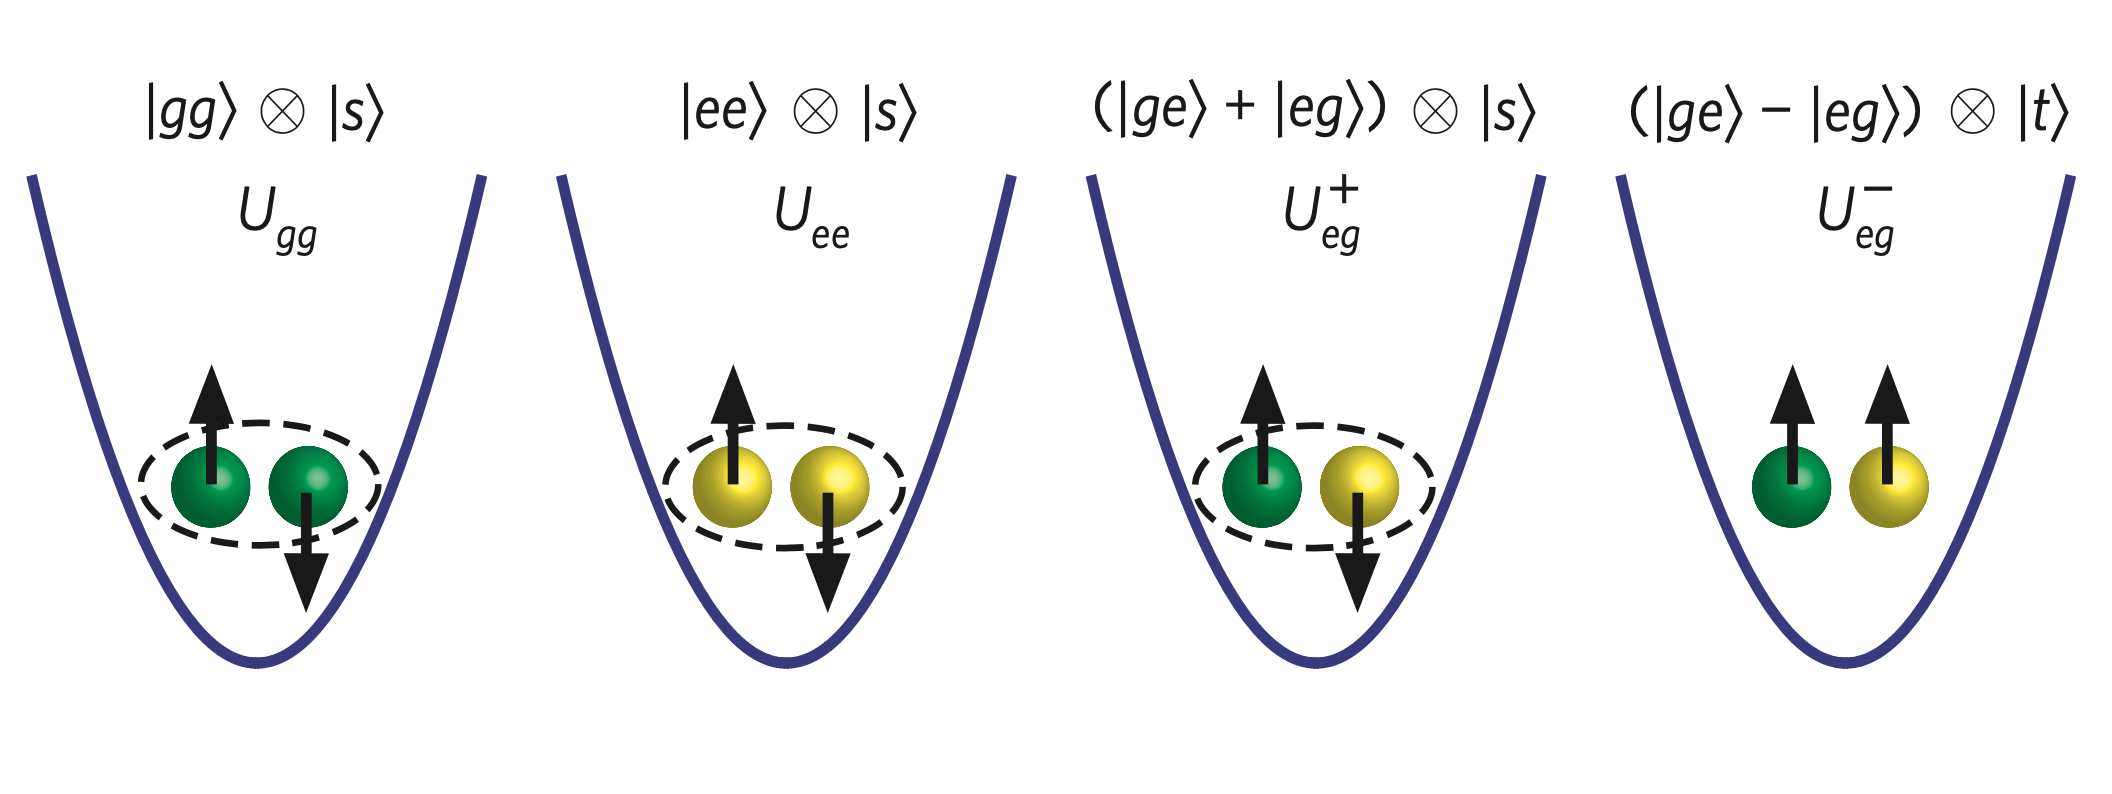
\includegraphics[width=0.7\textwidth]{eg.png}
    \bicaption{摘自SU(N)}{Reprinted from SU(N)}
    \label{eg}
\end{figure}
如果将$\hat{\rho}_{eg^\pm}$展开,我们得到不同轨道原子间的相互作用$\hat{V}_{eg}$分成了自旋交换与自旋守恒的两项:
\begin{equation}
\begin{aligned}
\hat{V}_{eg^+} &= g_{e g^+} \int \mathrm{d}^{3} \mathbf{r} \hat{\rho}_{eg^+}(\mathbf{r}) \hat{\rho}_{eg^+}(\mathbf{r})+g_{e g^-} \int \mathrm{d}^{3} \mathbf{r} \hat{\rho}_{eg^-}(\mathbf{r}) \hat{\rho}_{eg^-}(\mathbf{r})\\
\quad &= \frac{g_{e g}^{+}+g_{e g}^{-}}{2} \int \mathrm{d}^{3} \mathbf{r} \rho_{e}(\mathbf{r}) \rho_{g}(\mathbf{r}) \\ 
&\quad \quad + \frac{g_{e g}^{+}-g_{e g}^{-}}{2} \sum_{m m^{\prime}} \int \mathrm{d}^{3} \mathbf{r} \Psi_{g m}^{\dagger}(\mathbf{r}) \Psi_{e m^{\prime}}^{\dagger}(\mathbf{r}) \Psi_{g m^{\prime}}(\mathbf{r}) \Psi_{e m}(\mathbf{r})
\end{aligned}
\end{equation}
最后,将整个二次量子化哈密顿量在光晶格紧束缚近似下写为:
\begin{equation}
\begin{aligned}
\hat{H}=&-\sum_{\langle j, i\rangle \alpha, m} J_{\alpha}\left(c_{i \alpha m}^{\dagger} c_{j \alpha m}+\text { h.c. }\right)+\sum_{j, \alpha} \frac{U_{\alpha \alpha}}{2} n_{j \alpha}\left(n_{j \alpha}-1\right) \\
&+V \sum_{j} n_{j e} n_{j g}+V_{e x} \sum_{j, m, m^{\prime}} c_{j g m}^{\dagger} c_{j e m^{\prime}}^{\dagger} c_{j g m^{\prime}} c_{j e m}
\end{aligned}
\end{equation}
其中$\hat{n}_{j\alpha}=\sum_m \hat{n}_{j\alpha m}$,$V=\left(U_{e g}^{+}+U_{e g}^{-}\right) / 2$与$V_{ex}=\left(U_{e g}^{+}-U_{e g}^{-}\right) / 2$分别描述不同轨道原子间的自旋不变与自旋交换相互作用,其中:
\begin{equation}
U_{eg^\pm} = g_{eg^\pm} \int \mathrm{d}^{3} \mathbf{r} w_e^2(\mathbf{r})w_g^2(\mathbf{r})
\end{equation}
有了上述丰富的轨道间相互作用与核自旋SU(N)自由度,这一模型可以用来模拟众多凝聚态物理中强关联多体模型,比如近藤晶格模型、自旋链模型、自旋液体等。

紧接着于2014年,F. Scazza与合作者一起在${}^{173}$Yb体系中证实了上述自旋交换相互作用的存在。其思路如图~\ref{egexp}~所示:
\begin{figure}[!htbp]
    \centering
    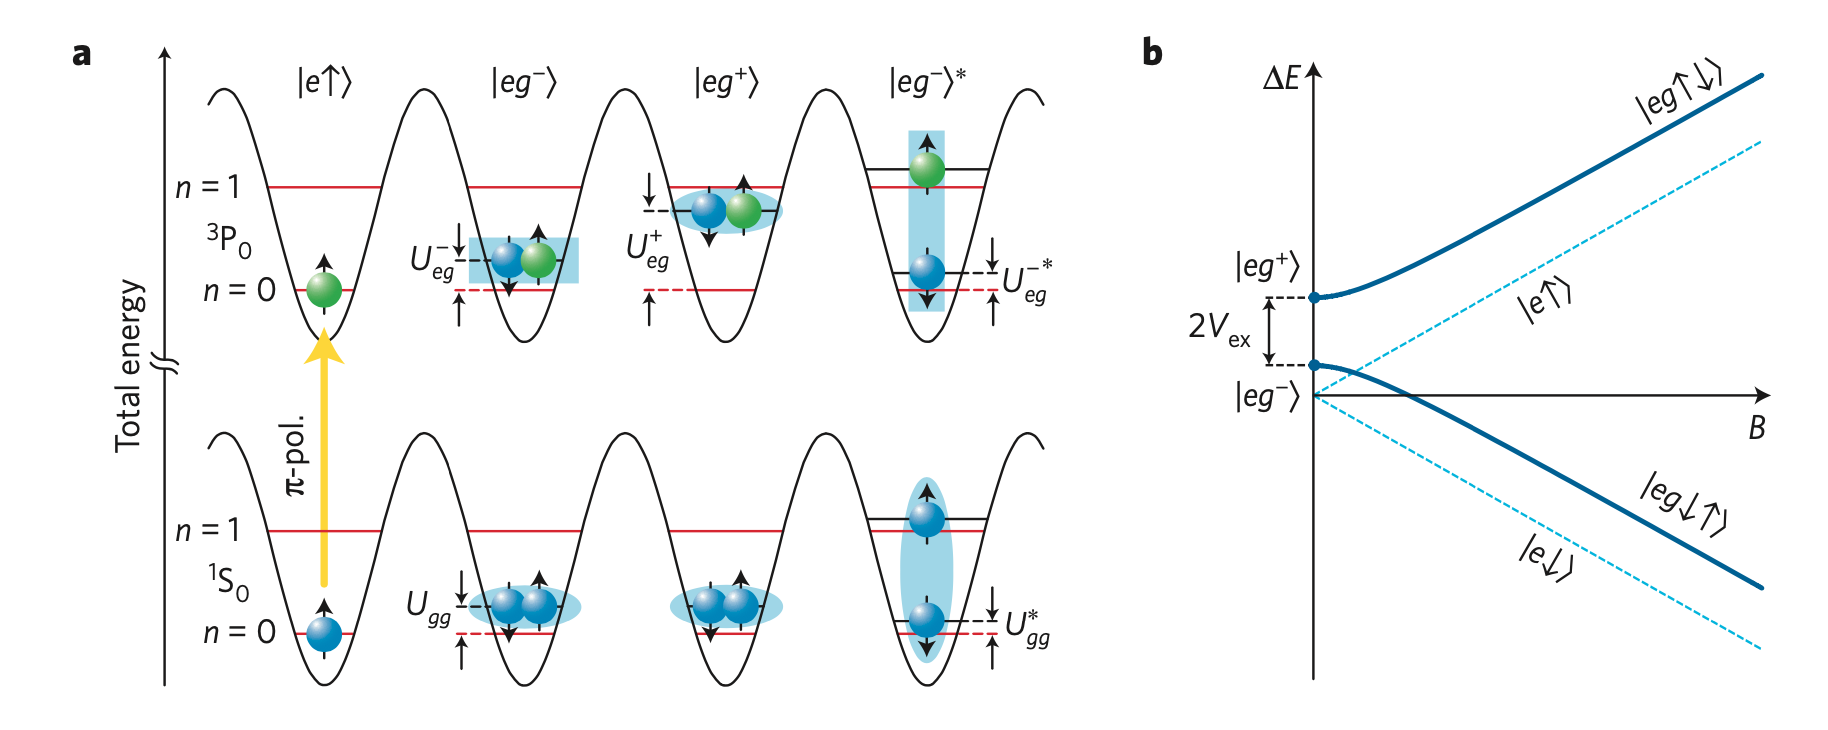
\includegraphics[width=0.7\textwidth]{egexp.png}
    \bicaption{摘自SU(N) exp}{Reprinted from SU(N) exp}
    \label{egexp}
\end{figure}
该实验选取不同电子排布($g({}^1S_0)$与$e({}^3P_0)$)的${}^{173}$Yb($I=5/2$)原子,束缚在较深(原子不能自由移动)的光晶格中,在每个格点里面,原子间的相互作用能为:
\begin{equation}
U_{X}=\frac{4 \pi \hbar^{2}}{m} a_{X} \int \mathrm{d}^{3} r w_{a}^{2}(\mathbf{r}) w_{b}^{2}(\mathbf{r})
\end{equation}
其中$X =gg, ee, eg^+, eg^−$代表不同状态的原子对。装载不同核自旋的$g$轨道原子到光晶格中,平均填充在$\bar{n}=1$与$\bar{n}=2$之间,这样导致部分格点内有一个原子,部分格点内有两个原子。对于有两个原子的格点,用激光将一个原子从g态激发到e态,末态有两个本征态$|eg^\pm\rangle$,本征能量为$U_{eg^\pm}$。如果在体系中加入沿$z$方向的磁场,导致$|eg^\pm\rangle$两态之间有非零的跃迁矩阵元,最终的哈密顿量为:
\begin{equation}
H_{e g}=\left(\begin{array}{cc}
U_{e g}^{+} & \Delta_{B} \\
\Delta_{B} & U_{e g}^{-}
\end{array}\right)
\end{equation}
其中$\Delta_{B}=\delta g m_{\mathrm{F}} \mu_{\mathrm{B}} B$,$\delta g$为核自旋朗德因子的差值,激光场下末态的本征能量为:
\begin{equation}
E_{1,2}=V \pm \sqrt{V_{\mathrm{ex}}^{2}+\Delta_{B}^{2}}
\end{equation}
本征波函数为$|eg^\pm\rangle$两态的线性叠加。

通过观测不同磁场下的共振谱,得到不同磁场下末态的能量,如图~\ref{egd}~
\begin{figure}[!htbp]
    \centering
    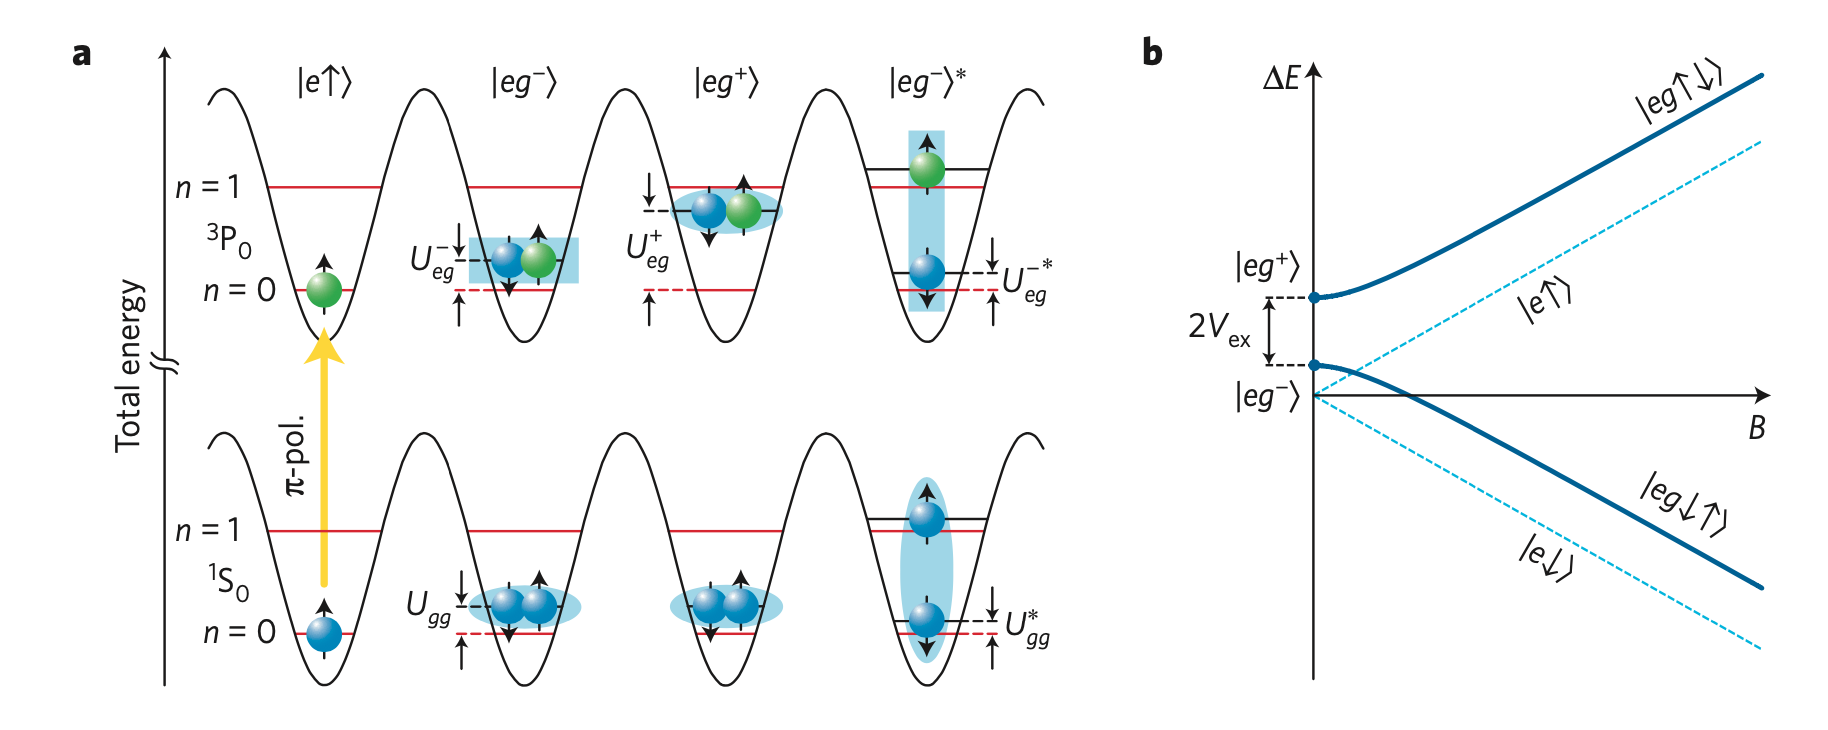
\includegraphics[width=0.7\textwidth]{egexp.png}
    \bicaption{摘自SU(N) exp}{Reprinted from SU(N) exp}
    \label{egd}
\end{figure}
拟合实验中不同磁场喜爱测到的共振峰的位置,最终得到的裸的散射长度为:{\color{red}散射长度数据}。进一步作者将光晶格的深度放浅让原子可以在晶格中动起来,研究演化一段时间后自旋极化的变化来直接观测到了自旋交换相互作用。

与此同时,来自研究者也分别在中观测到了自旋交换相互作用{\color{red}Sr与慕尼黑}。


\subsection{自旋交换理论}

进一步地,上述实验中发现的裸的自旋交换相互作用都比较小,用来做近藤物理的量子模拟尚有欠缺。因此理论研究者提出利用束缚诱导共振来调节自旋交换相互作用。具体地,



\section{极化子理论与实验}

极化子是一个杂质物理中比较古老的概念。早在固体物理中就有研究大极化子与小极化子\cite{landau1933bewegung,pekar1946autolocalization,frohlich1950xx,frohlich1954electrons,feynman1955slow,mahanmany},对应的是电子在晶格中运动,电子的单粒子性质被晶格声子激发所修饰,改变其有效质量、寿命等。严格说属于玻色极化子。如果将背景原子改为多体费米体系,就得到费米极化子。理论上,极化子是典型的费米液体。近年来,随着冷原子中Imblanced 费米混合气体的制备,极化子作为其中的极端体系,进入研究者的视野,结合冷原子体系特有的控制、操控、观测能力,极化子的研究迎来新的阶段,我们将围绕相关研究的实验与理论展开。
\begin{figure}[!htbp]
    \centering
    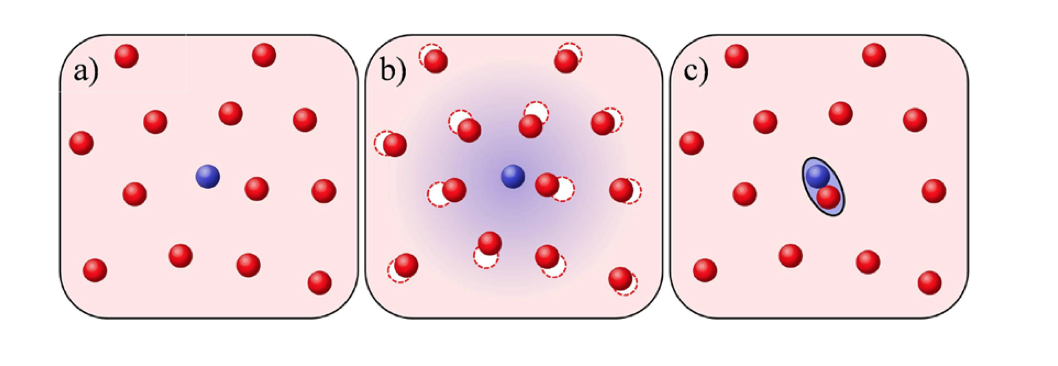
\includegraphics[width=0.7\textwidth]{chap1fp.png}
    \bicaption{摘自SU(N) exp}{Reprinted from SU(N) exp}
    \label{fp}
\end{figure}

\subsection{极化子实验}
超冷原子中极化子物理研究的启发来自于population-imblanced混合费米气体。其中少数原子成为杂质,多数原子构成背景。费米极化子最早的直接实验证据来自MIT研究组\cite{Schirotzekobservation}。实验上制备${}^6$Li。
\begin{figure}[!htbp]
    \centering
    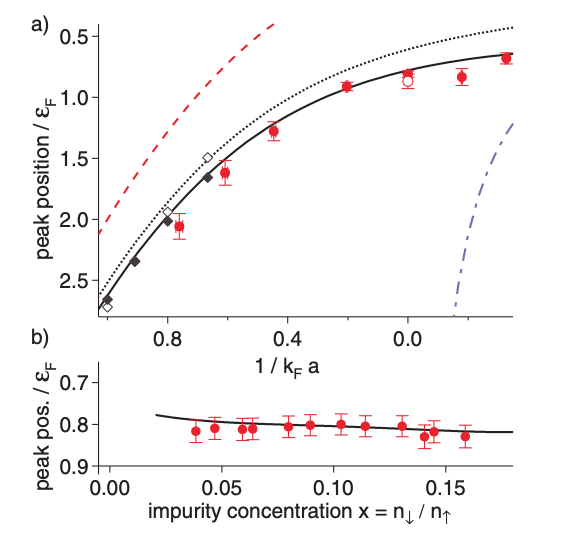
\includegraphics[width=0.7\textwidth]{chap1fpE.png}
    \bicaption{摘自SU(N) exp}{Reprinted from SU(N) exp}
    \label{fpE}
\end{figure}
进一步分析能谱,提取出准粒子剩余
\begin{figure}[!htbp]
    \centering
    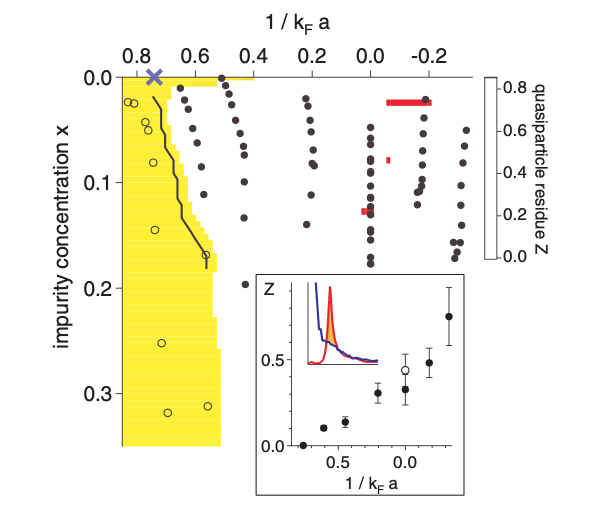
\includegraphics[width=0.7\textwidth]{chap1fpZ.png}
    \bicaption{摘自SU(N) exp}{Reprinted from SU(N) exp}
    \label{fpZ}
\end{figure}

后续实验进一步观测到upper branch\cite{kohstall2012metastability,}:
\begin{figure}[!htbp]
    \centering
    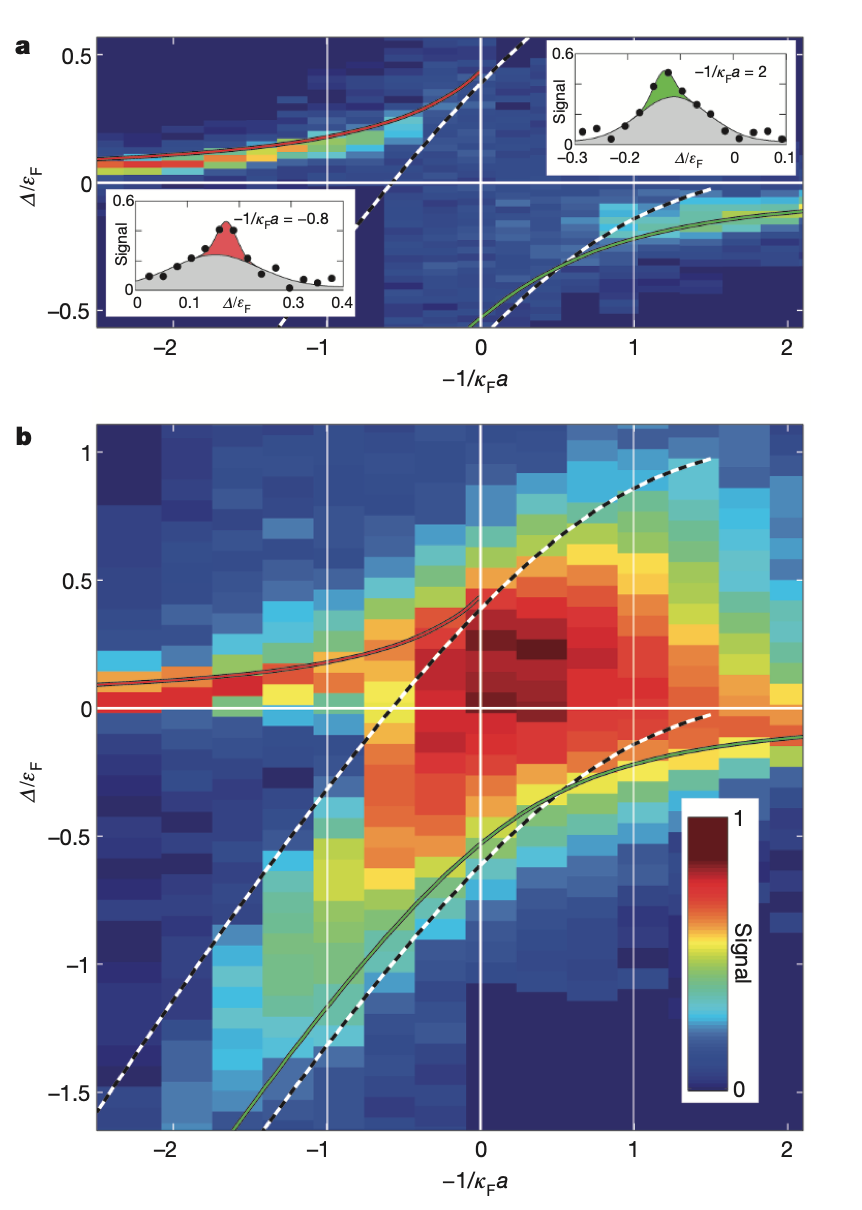
\includegraphics[width=0.7\textwidth]{chap1upfp.png}
    \bicaption{摘自SU(N) exp}{Reprinted from SU(N) exp}
    \label{upfp}
\end{figure}

降低维度观测到2D极化子low与up\cite{koschorreck2012attractive}。
\begin{figure}[!htbp]
    \centering
    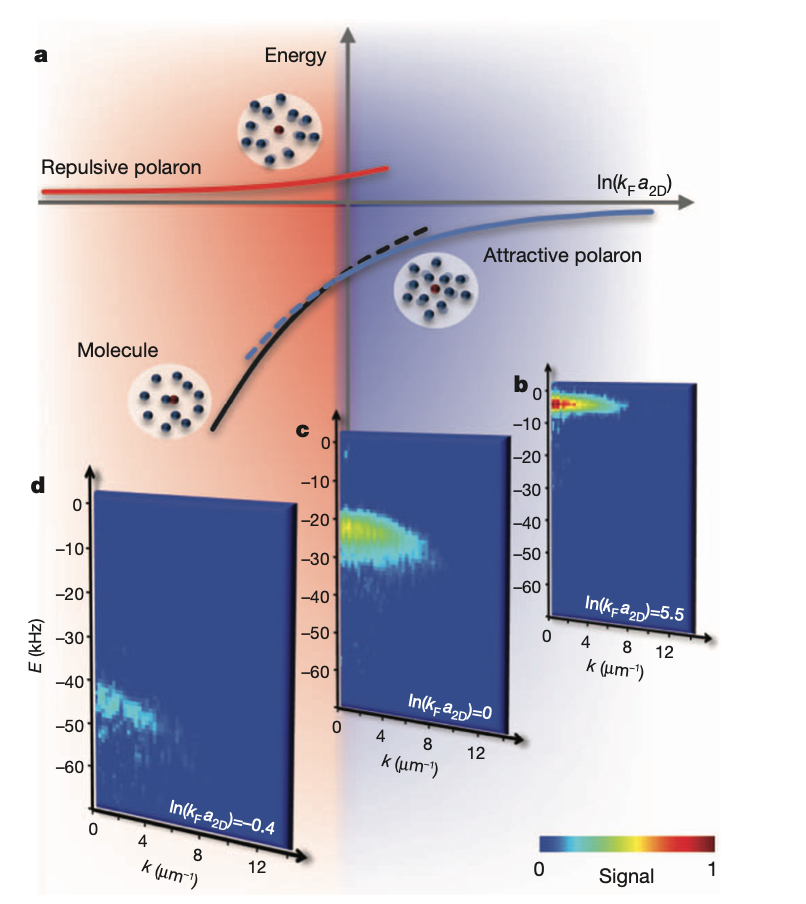
\includegraphics[width=0.7\textwidth]{chap12dfp.png}
    \bicaption{摘自SU(N) exp}{Reprinted from SU(N) exp}
    \label{2dfp}
\end{figure}

超快Ramesy spectroscopy
\begin{figure}[!htbp]
    \centering
    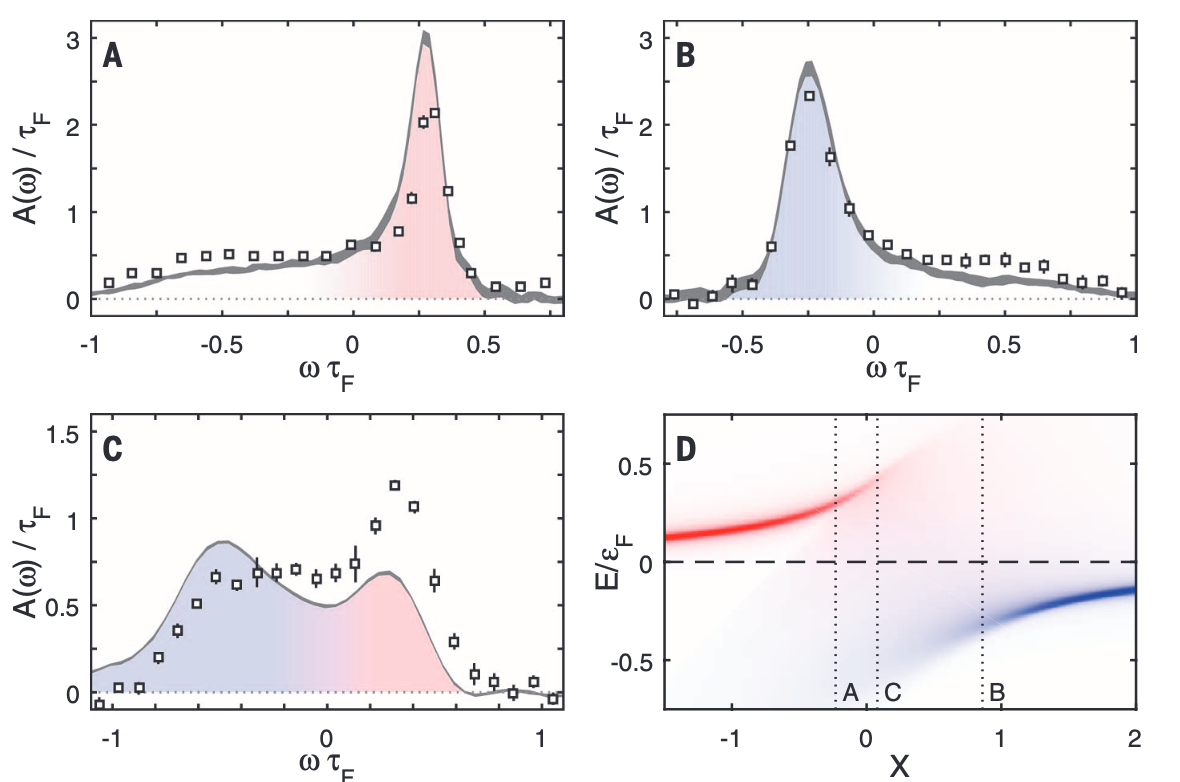
\includegraphics[width=0.7\textwidth]{chap1fpultra.png}
    \bicaption{摘自SU(N) exp}{Reprinted from SU(N) exp}
    \label{fpultra}
\end{figure}

有限温度polaron
\begin{figure}[!htbp]
    \centering
    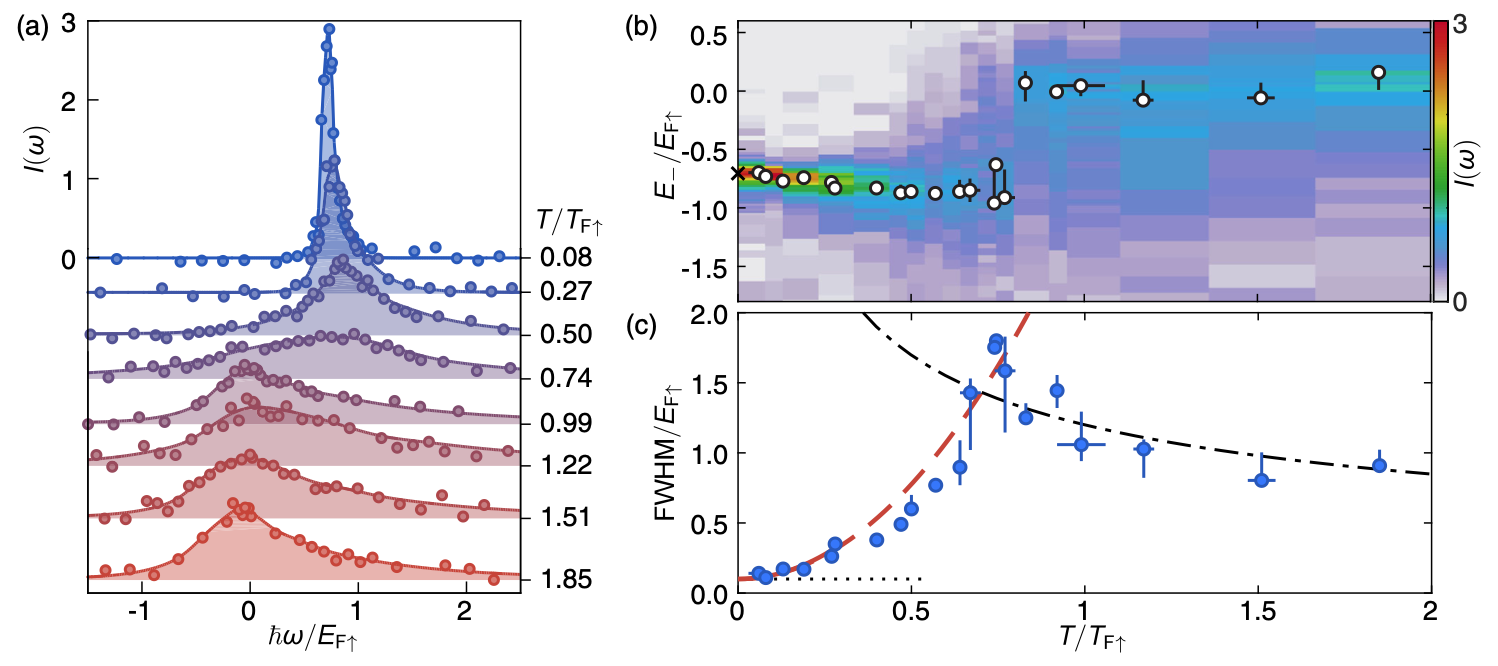
\includegraphics[width=0.7\textwidth]{chap1fpT.png}
    \bicaption{摘自SU(N) exp}{Reprinted from SU(N) exp}
    \label{fpT}
\end{figure}




\subsection{极化子理论}
理论方面关注整个相互作用可调区间,冷原子中费米极化子的研究最早可追溯到Chevy变分波函数,在整个相互作用区间都很好的成立。


V-ph
chevy
3D
2D
1D

RF

MC

拓扑极化子

最新进展














